\section{Architecture de la solution (C4 et ADR)}
\label{chap:architecture}

Cette section présente l'architecture logicielle et d'infrastructure retenue pour la plateforme SOYAFF, selon les trois premiers niveaux du modèle C4 (contexte, conteneurs, composants), complétés par une vue de déploiement de l'infrastructure de production.

\subsection{Vue de contexte}
\label{sec:c4_contexte}
La Figure~\ref{fig:c4_contexte} situe la plateforme SOYAFF parmi les systèmes avec lesquels elle interagit : les trois rôles utilisateurs, l'API Claude d'Anthropic pour le traitement cloud des requêtes non sensibles (\texttt{EF-RAG-03}), les fichiers Excel legacy servant de source à l'import historique (\texttt{EF-ETL-01}), et l'application \texttt{kiri.app} déjà en usage, dont le périmètre disjoint est explicitement représenté (§\ref{sec:recueil}).

\begin{figure}[H]
    \centering
    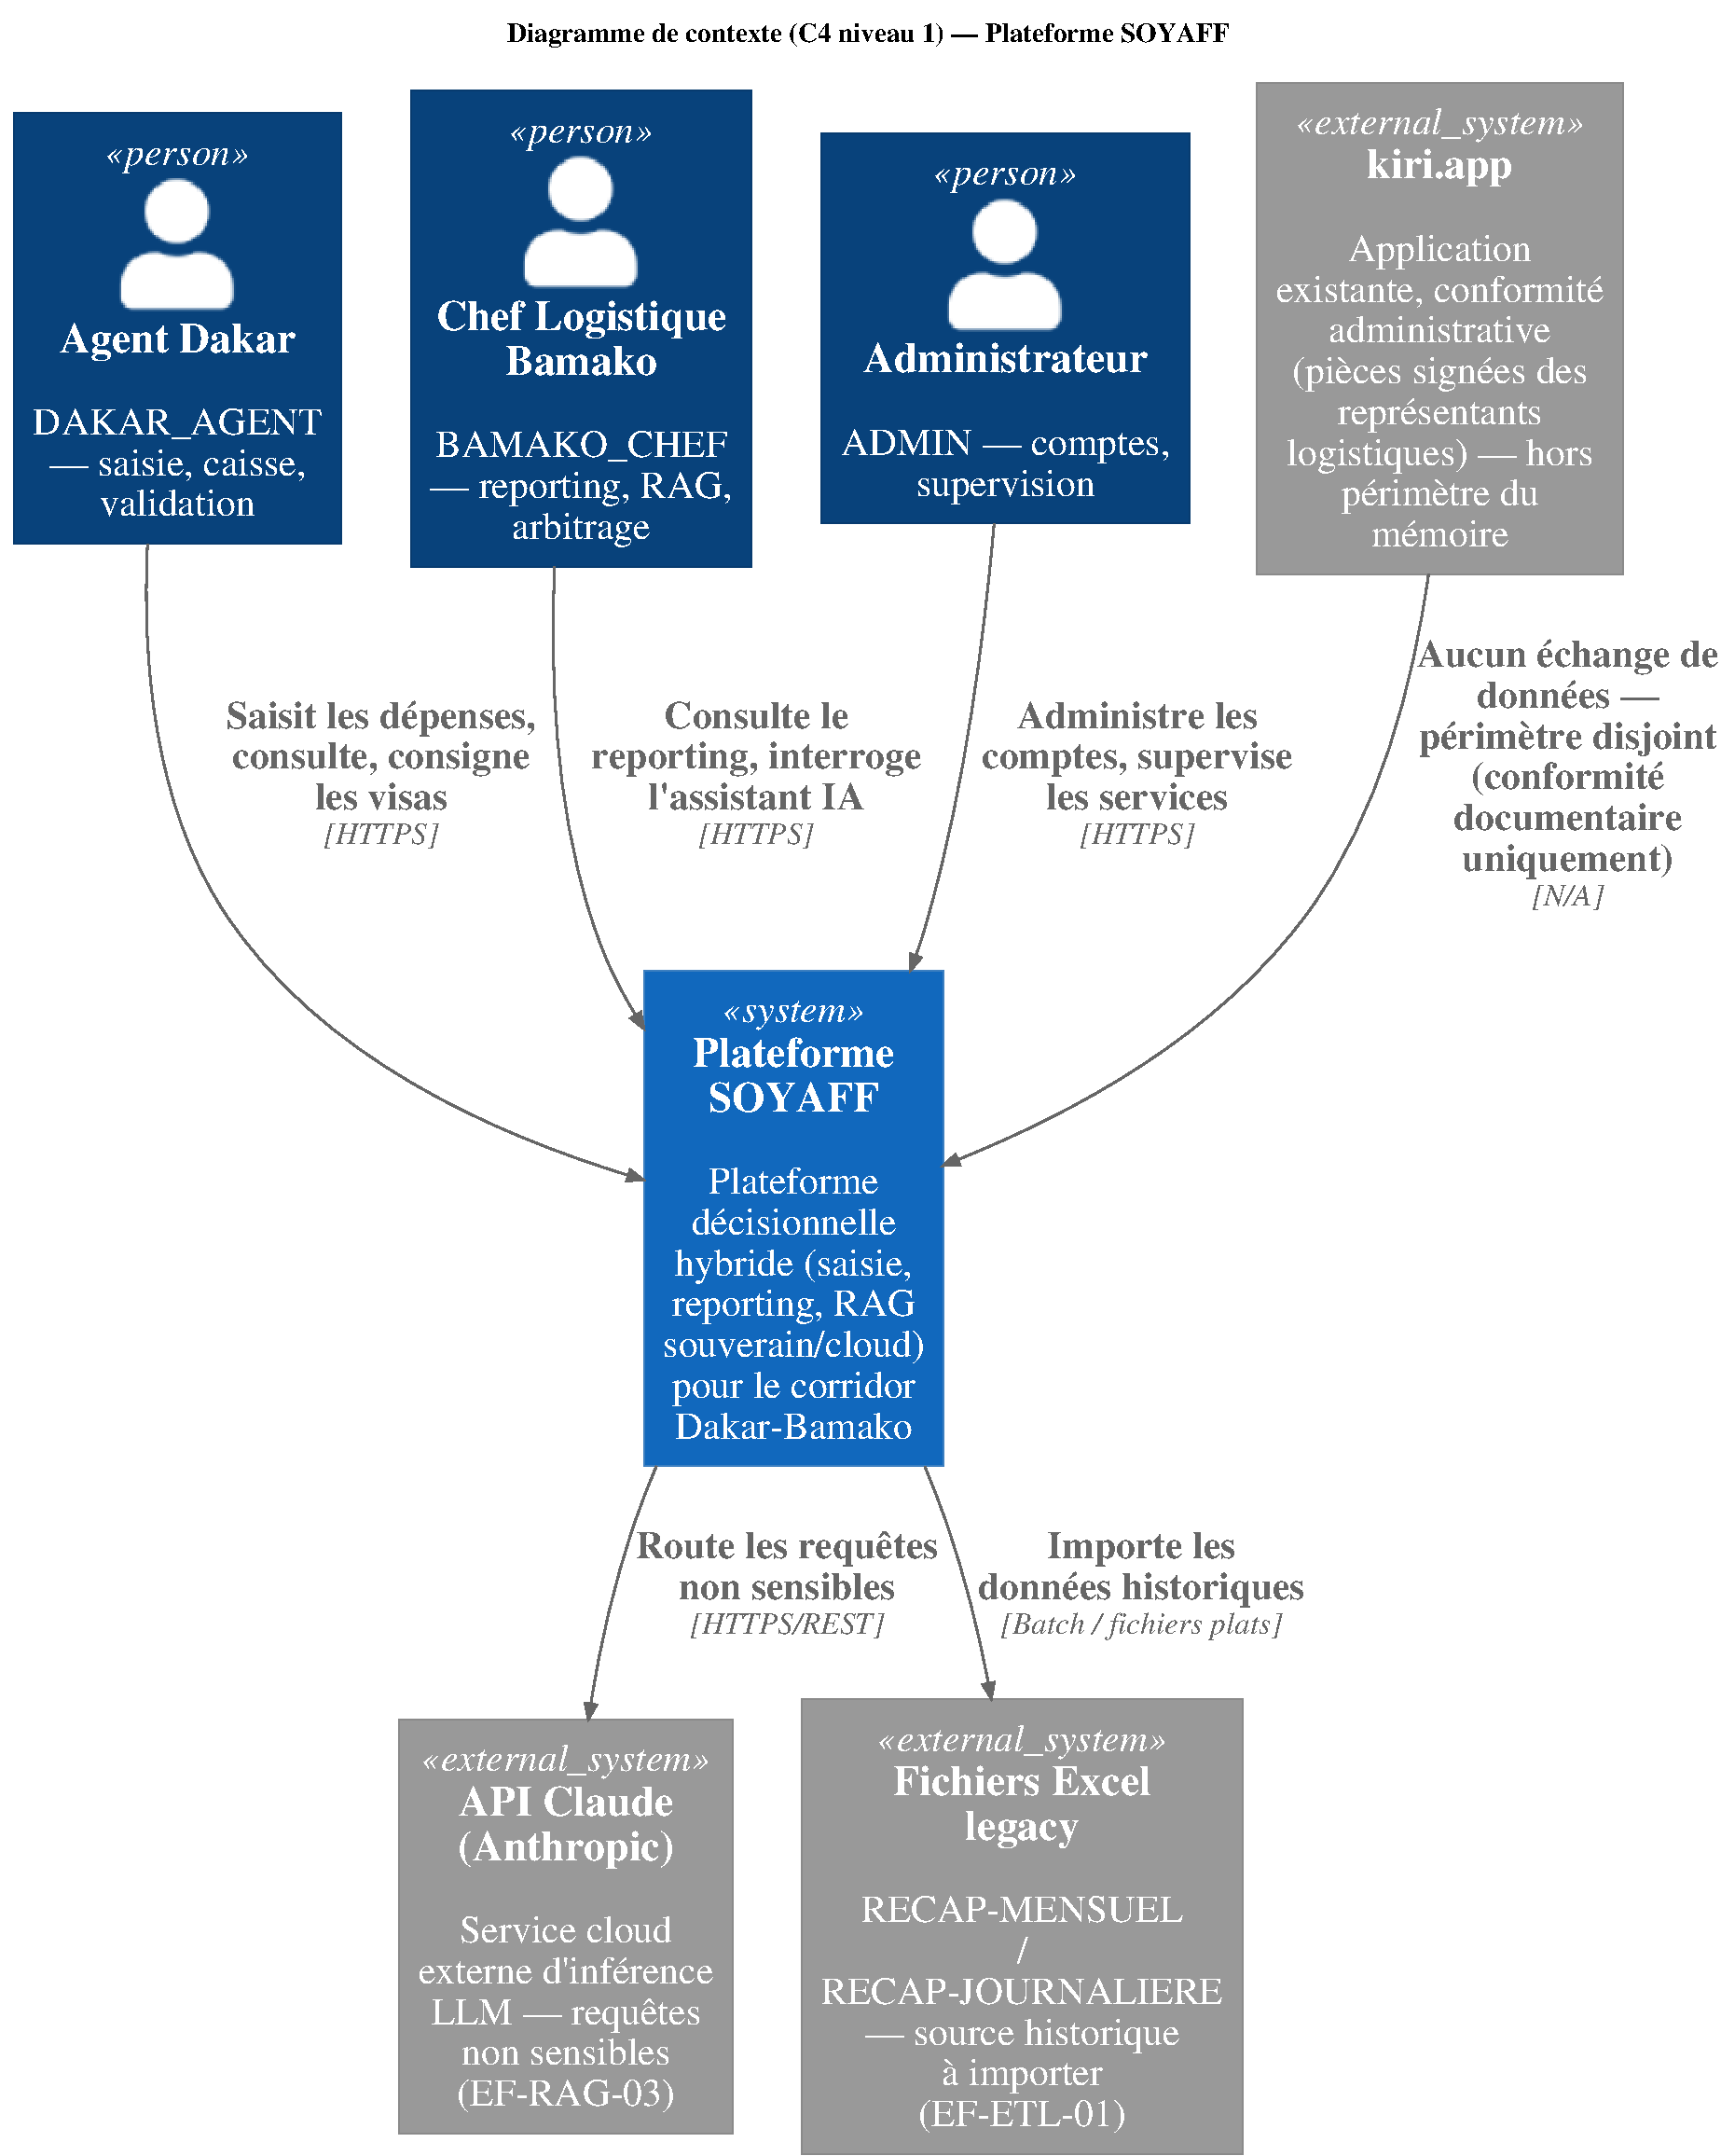
\includegraphics[width=\textwidth,height=0.88\textheight,keepaspectratio]{figures/fig_c4_contexte.pdf}
    \caption{Diagramme de contexte (C4 niveau 1), plateforme SOYAFF}
    \label{fig:c4_contexte}
    \source{Schéma de l'auteur}
\end{figure}

\subsection{Vue de conteneurs}
\label{sec:c4_conteneurs}
La Figure~\ref{fig:c4_conteneurs} détaille les conteneurs applicatifs déployés au sein du périmètre souverain de la plateforme. Le point d'entrée unique du module conversationnel est l'orchestrateur n8n, qui analyse la sensibilité de chaque requête et la route vers le service RAG local (FastAPI, Ollama/Mistral) ou vers l'API Claude cloud, conformément à \texttt{EF-RAG-03}. La conversation est journalisée en base (\texttt{EF-RAG-05}) indépendamment du chemin emprunté.

La frontière «\,périmètre souverain\,» tracée sur la figure n'est pas cosmétique : elle délimite l'ensemble des conteneurs au sein desquels les données métier ne quittent jamais l'infrastructure maîtrisée. Seul le chemin cloud (API Claude) la franchit, et uniquement pour des requêtes préalablement classées non sensibles par l'orchestrateur. Cette étanchéité conditionne la validité des exigences \texttt{ENF-SOUV-01} et \texttt{ENF-SOUV-02}.

\begin{figure}[H]
    \centering
    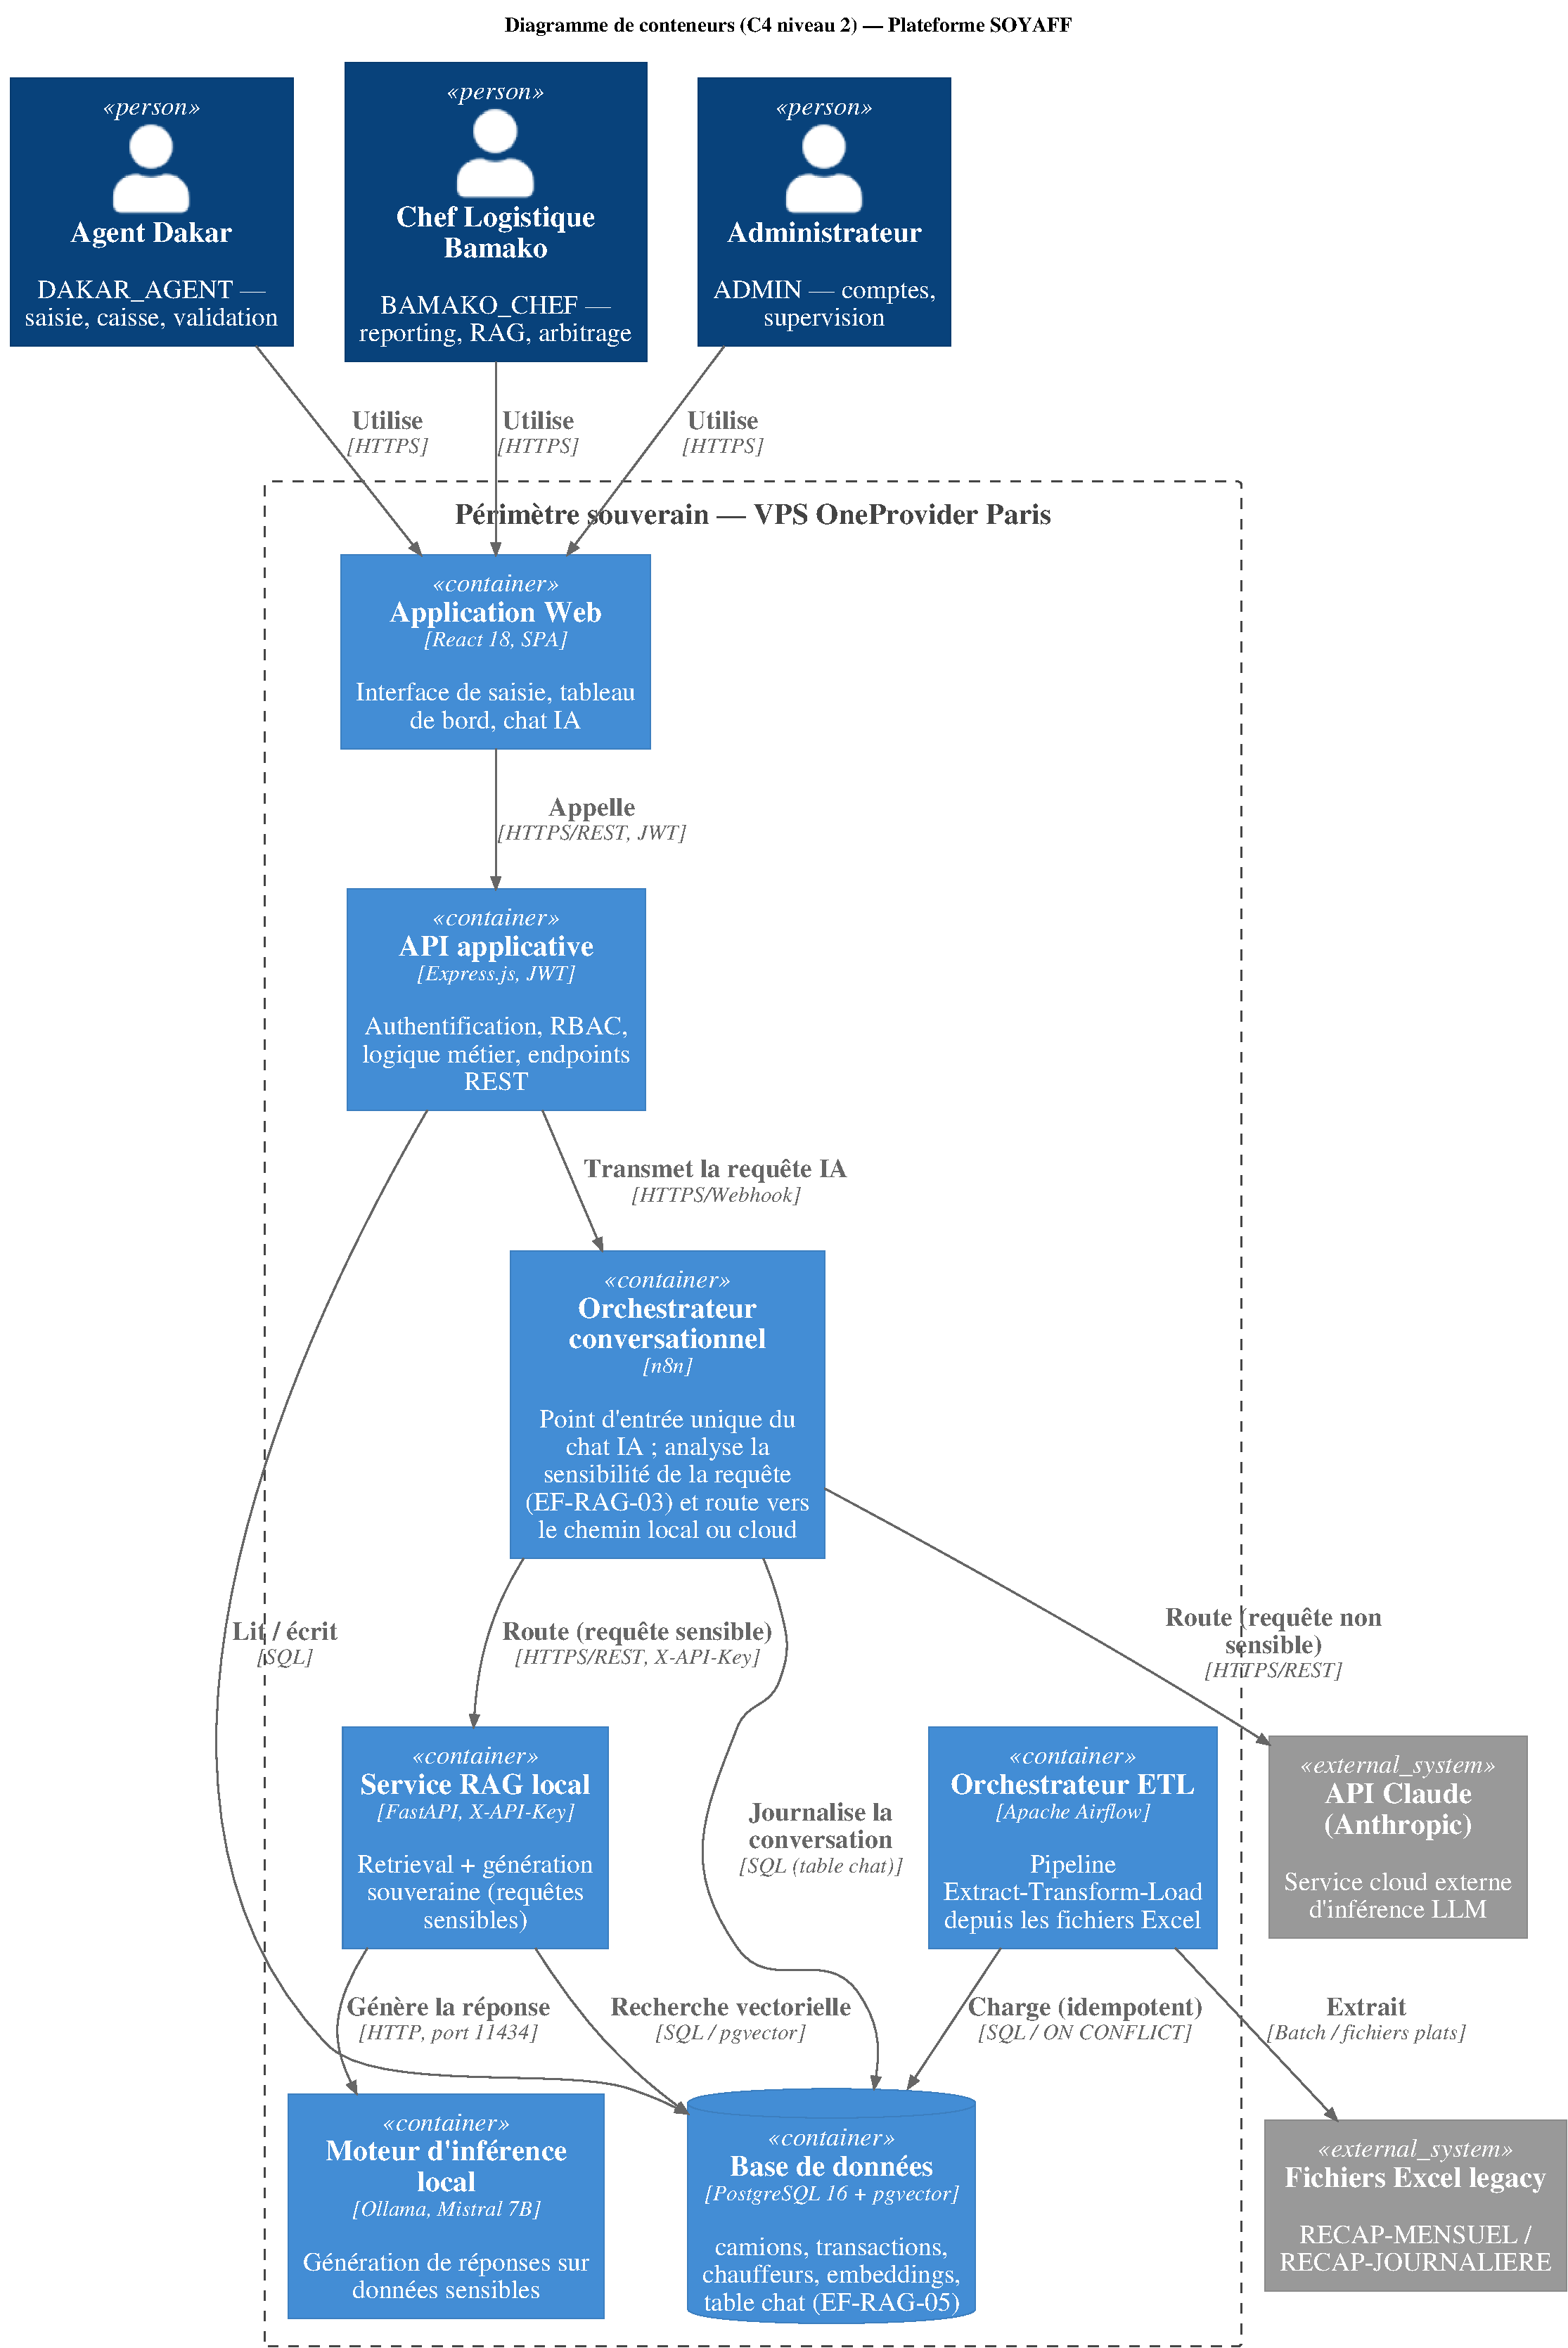
\includegraphics[width=\textwidth,height=0.88\textheight,keepaspectratio]{figures/fig_c4_conteneurs.pdf}
    \caption{Diagramme de conteneurs (C4 niveau 2), plateforme SOYAFF}
    \label{fig:c4_conteneurs}
    \source{Schéma de l'auteur}
\end{figure}

\subsection{Vue de composants : service RAG local}
\label{sec:c4_composants}
Nous ne détaillons le niveau 3 (composants) que pour le conteneur le plus significatif. La Figure~\ref{fig:c4_composants_rag} isole donc les composants internes du service RAG local (FastAPI) : le gestionnaire de requêtes, un composant de réponses SQL directes (comptages, solde), le module de retrieval (filtres SQL puis repli vectoriel \texttt{all-MiniLM-L6-v2}), le constructeur de contexte et le client d'inférence. Les questions de comptage, de solde et de total sont servies sans modèle de langage ; les autres sont confiées à Mistral~7B. Cette vue met aussi en évidence deux écarts à l'exigence de maintenabilité (\texttt{ENF-MAINT-01}, \texttt{ENF-MAINT-02}), détaillés au §\ref{sec:ia_dettes}.

\begin{figure}[H]
    \centering
    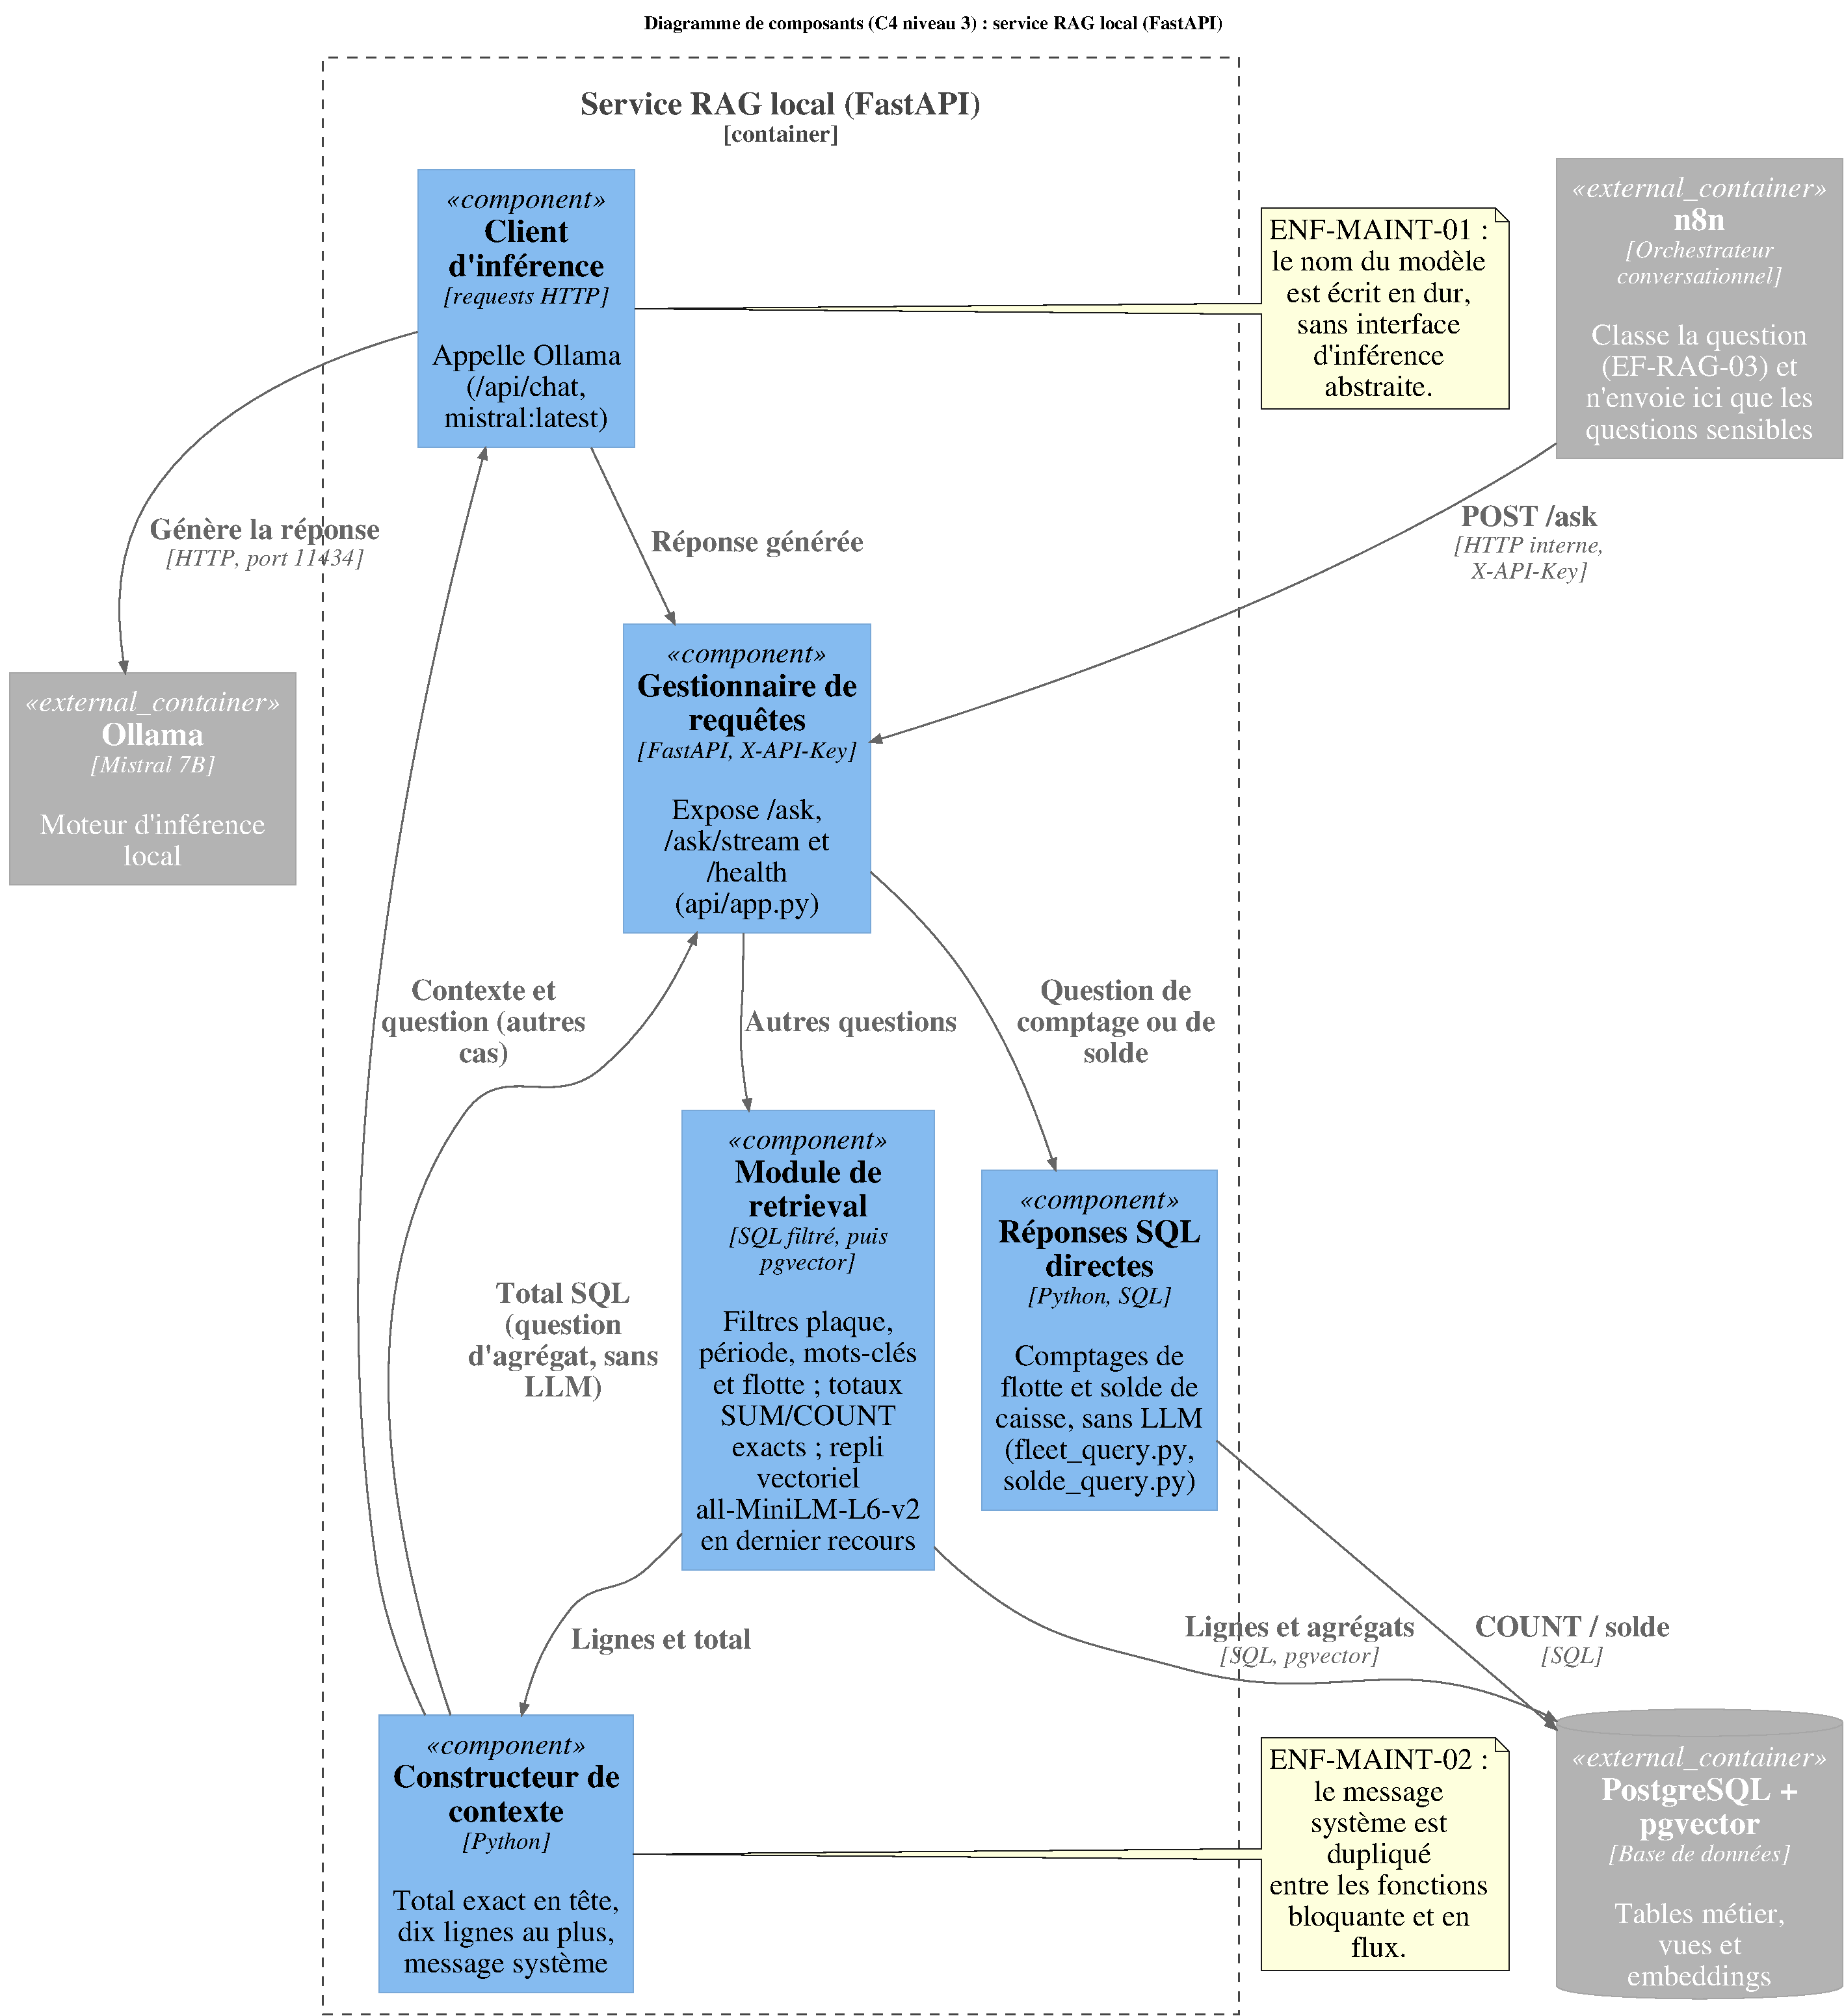
\includegraphics[width=\textwidth,height=0.88\textheight,keepaspectratio]{figures/fig_c4_composants_rag.pdf}
    \caption{Diagramme de composants (C4 niveau 3), service RAG local}
    \label{fig:c4_composants_rag}
    \source{Schéma de l'auteur}
\end{figure}

\subsection{Déploiement}
\label{sec:deploiement}
La Figure~\ref{fig:deploiement} décrit l'infrastructure de production : tous les conteneurs applicatifs, IA, ETL et de supervision sont hébergés sur un seul serveur dédié, ce qui soutient directement l'hypothèse de frugalité H1 (\texttt{ENF-FRUG-01}). Le trafic des clients passe par Cloudflare, chiffré de bout en bout (ADR-05). Quatre services externes complètent le schéma : l'API Anthropic pour le chemin cloud, GitLab.com pour les dépôts et les pipelines, Telegram pour les alertes et l'espace de sauvegarde de l'hébergeur. Pour rester lisible, le schéma est présenté en deux vues : la vue d'ensemble du serveur et de ses flux externes (Figure~\ref{fig:deploiement}), puis le détail des conteneurs du réseau Docker (Figure~\ref{fig:deploiement_docker}).

\begin{landscape}
\begin{figure}[p]
    \centering
    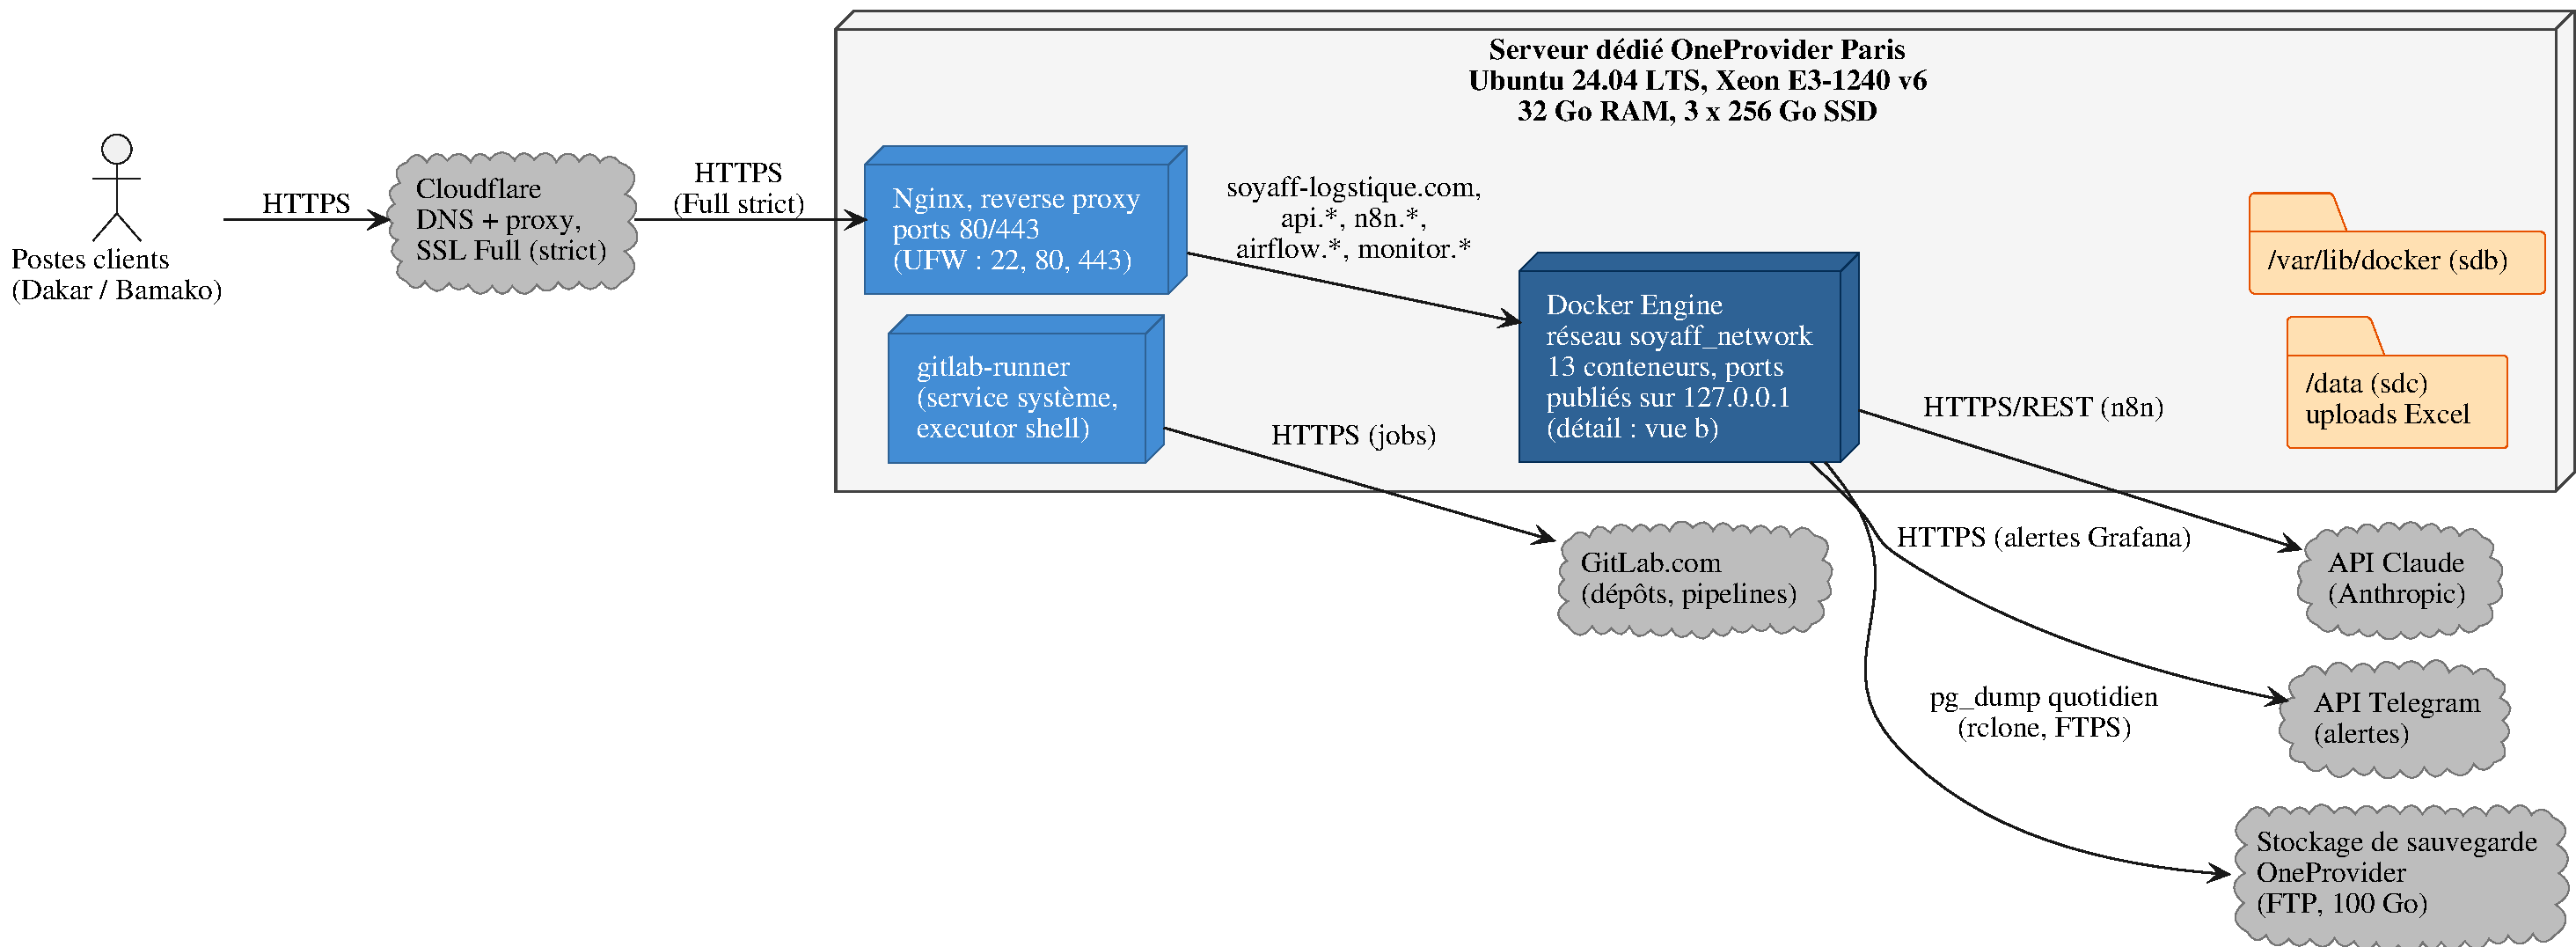
\includegraphics[width=\linewidth,height=0.86\textheight,keepaspectratio]{figures/fig_deploiement_vue.pdf}
    \caption{Diagramme de déploiement (1/2) : serveur de production et services externes}
    \label{fig:deploiement}
    \source{Schéma de l'auteur}
\end{figure}
\begin{figure}[p]
    \centering
    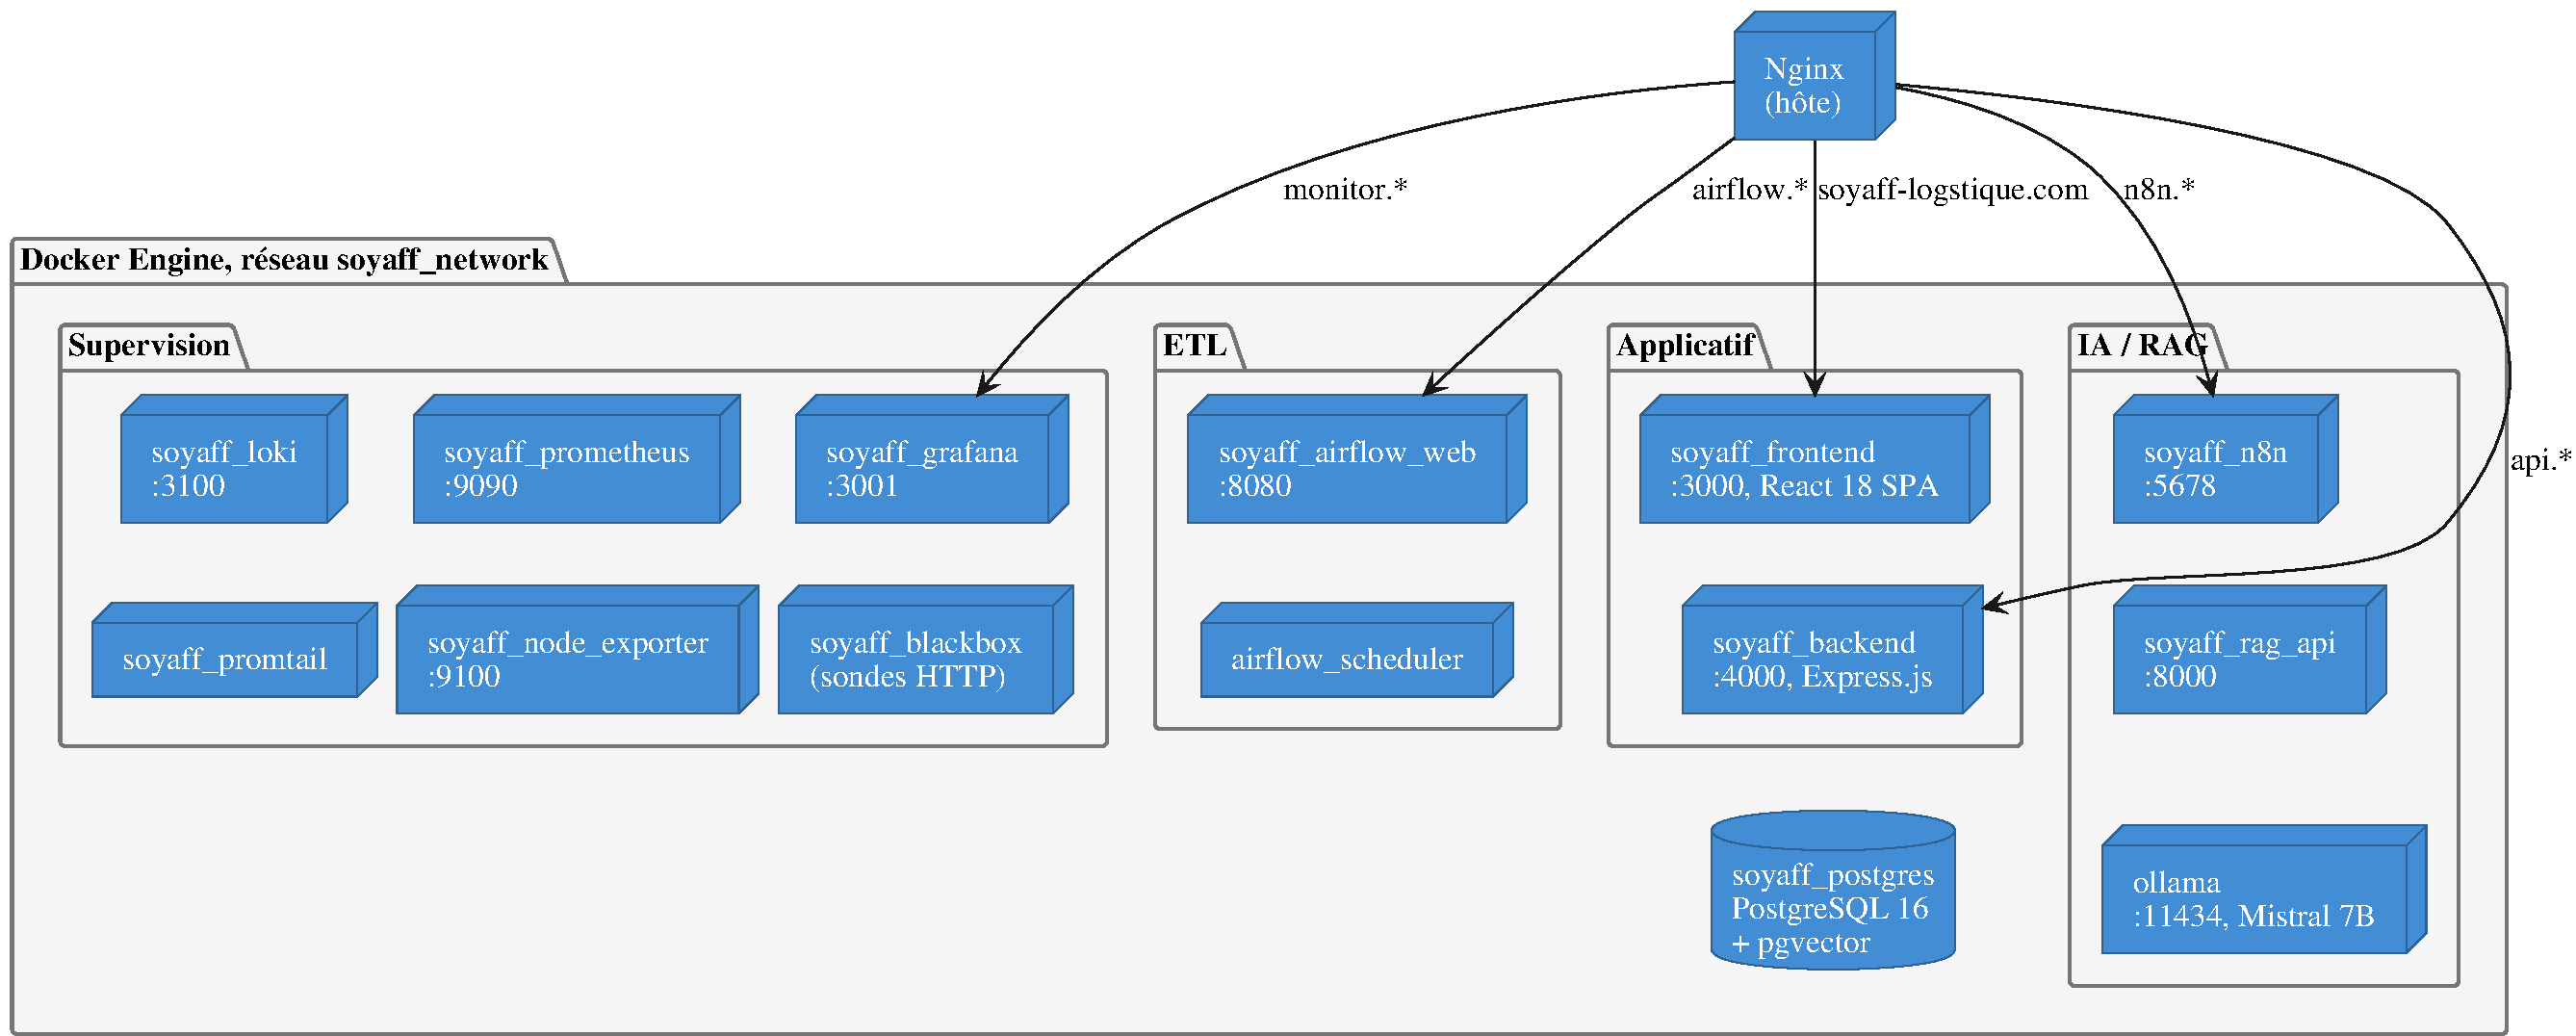
\includegraphics[width=\linewidth,height=0.86\textheight,keepaspectratio]{figures/fig_deploiement_docker.pdf}
    \caption{Diagramme de déploiement (2/2) : conteneurs du réseau Docker \texttt{soyaff\_network}}
    \label{fig:deploiement_docker}
    \source{Schéma de l'auteur}
\end{figure}
\end{landscape}

\subsection{Registre des décisions architecturales (ADR)}
\label{sec:adr}
Les vues précédentes décrivent l'architecture retenue. Cette section en justifie les décisions sous forme d'Architecture Decision Records (ADR) : contexte, option retenue, conséquences (bénéfices comme dettes assumées), et alternatives écartées.

\subsubsection*{ADR-01 : Orchestration ETL par Apache Airflow}
\textbf{Contexte.} Le pipeline d'ingestion des fichiers Excel hétérogènes (\texttt{RECAP-MENSUEL}, \texttt{RECAP-JOURNALIERE}) exige planification, idempotence et gestion de \textit{backfill} en environnement à connectivité intermittente, propre au corridor Dakar--Bamako (§2.2.3). Le choix de l'orchestrateur devait concilier maturité technique et indépendance vis-à-vis des éditeurs commerciaux (§2.2.4).

\textbf{Décision.} Apache Airflow est retenu comme orchestrateur ETL, modélisant le pipeline sous forme de DAG Python idempotents, la déduplication reposant sur la clé \texttt{source\_key} (\texttt{ON CONFLICT DO NOTHING}).

\textbf{Conséquences.} \textit{Positives} : licence Apache~2.0 garantissant une indépendance totale vis-à-vis d'un éditeur ; large éventail de connecteurs matures pour sources hétérogènes (Excel, PDF, PostgreSQL) ; gestion native du \textit{backfill}. \textit{Négatives} : courbe d'apprentissage modérée à difficile ; empreinte ressources plus lourde qu'un ordonnanceur léger de type \textit{cron}.

\textbf{Alternatives écartées.} Prefect et Dagster, tous deux adossés à un modèle commercial cloud qui réintroduirait précisément la dépendance logicielle exogène que l'architecture cherche à éviter (§2.2.4).

\textbf{Exigences / hypothèses liées.} \texttt{EF-ETL-01}, \texttt{EF-ETL-02}, \texttt{ENF-VOL-01}, H4.

\subsubsection*{ADR-02 : Routage hybride cloud/local par sensibilité}
\textbf{Contexte.} Une tension oppose la souveraineté des données sensibles (identités des chauffeurs, montants, opérations financières) à la puissance de calcul disponible localement pour l'inférence LLM, le serveur ne disposant d'aucun GPU dédié (§2.4). Le besoin décisionnel exprimé par \texttt{EF-RAG-01/02} exige néanmoins un agent conversationnel capable de traiter des requêtes analytiques complexes.

\textbf{Décision.} La sensibilité de chaque requête est classifiée en amont par un nœud d'analyse par mots-clés au sein du workflow n8n, qui route ensuite vers l'un de deux chemins : le service RAG local (FastAPI + pgvector + Ollama/Mistral, aucune sortie réseau) pour les requêtes sensibles, l'API Claude cloud pour les requêtes non sensibles.

\textbf{Conséquences.} \textit{Positives} : conformité déclarative à \texttt{ENF-SOUV-01} pour le périmètre classé sensible ; accès à la puissance d'un LLM cloud pour les requêtes complexes sans investissement GPU. \textit{Négatives} : la classification par mots-clés reste une heuristique et non un mécanisme certifié, avec un risque résiduel de faux négatif (requête sensible mal classée et routée vers le cloud) ; le chemin local ne repose pas encore sur une interface d'inférence abstraite (écart \texttt{ENF-MAINT-01}, §\ref{sec:c4_composants}). \textit{Résolu} (section~\ref{chap:ia_rag}, §\ref{sec:ia_routage}) : le workflow n8n est versionné et le routage a été vérifié dans les deux sens ; une mention d'identité (chauffeur, plaque) reste désormais locale même dans une question d'agrégat ; l'outil SQL de l'agent cloud utilise un rôle PostgreSQL en lecture seule, sans accès aux données des chauffeurs.

\textbf{Alternatives écartées.} Tout-cloud, écarté comme incompatible avec \texttt{ENF-SOUV-01} et H2 ; tout-local, écarté faute de puissance suffisante pour satisfaire \texttt{ENF-PERF-02/03} sur les requêtes analytiques complexes avec le matériel disponible.

\textbf{Exigences / hypothèses liées.} \texttt{EF-RAG-01} à \texttt{05}, \texttt{ENF-SOUV-01}, \texttt{ENF-SOUV-02}, H2.

\subsubsection*{ADR-03 : Déploiement mono-hôte sur serveur dédié unique}
\textbf{Contexte.} La contrainte budgétaire d'une PME subsaharienne (H1) doit être mise en balance avec le nombre croissant de services nécessaires à la plateforme (applicatif, IA, ETL, observabilité, CI/CD).

\textbf{Décision.} L'intégralité de la plateforme (quatorze conteneurs Docker) est hébergée sur un unique serveur dédié (OneProvider Paris, Xeon E3-1240 v6, 32~Go RAM, 3~$\times$~256~Go SSD), orchestrés via Docker Engine sur un réseau applicatif unique (\texttt{soyaff\_network}).

\textbf{Conséquences.} \textit{Positives} : coût d'infrastructure minimal, compatible avec \texttt{ENF-FRUG-01} ; simplicité opérationnelle d'un point d'administration unique. \textit{Négatives} : point de défaillance unique (\textit{SPOF}), donc aucune haute disponibilité : une panne matérielle ou une saturation de ressource affecte simultanément l'ensemble des services ; absence de scalabilité horizontale native. Cette dette est assumée explicitement et reprise à la section~\ref{chap:discussion}.

\textbf{Alternatives écartées.} Déploiement multi-nœuds ou infrastructure managée (Kubernetes cloud, bases de données managées), au coût mensuel incompatible avec \texttt{ENF-FRUG-01} et la réalité budgétaire d'une PME du secteur.

\textbf{Exigences / hypothèses liées.} \texttt{ENF-FRUG-01}, \texttt{ENF-DISP-02}, H1.

\subsubsection*{ADR-04 : PostgreSQL + pgvector plutôt qu'une base vectorielle dédiée}
\textbf{Contexte.} Le RAG local requiert un stockage d'embeddings vectoriels pour la recherche par similarité, en complément du stockage relationnel déjà nécessaire aux données métier (transactions, camions, chauffeurs).

\textbf{Décision.} Le stockage relationnel et vectoriel est mutualisé au sein d'un unique moteur PostgreSQL~16 étendu par \texttt{pgvector}, plutôt que de déployer une base vectorielle dédiée.

\textbf{Conséquences.} \textit{Positives} : un conteneur de moins à opérer et sécuriser, cohérent avec l'ADR-03 ; cohérence transactionnelle native entre données métier et embeddings, source de vérité unique facilitant la sauvegarde (\texttt{EF-ADM-03}) ; requêtes hybrides SQL/vectorielles en une seule transaction. \textit{Négatives} : performances de recherche vectorielle a priori inférieures à celles d'une base spécialisée sur de très gros volumes, ce qui n'est pas discriminant à la volumétrie actuelle de SOYAFF (\texttt{ENF-VOL-02}).

\textbf{Alternatives écartées.} Pinecone, écarté comme service SaaS propriétaire incompatible avec la souveraineté visée par H2 ; Qdrant ou Weaviate en conteneur dédié, fonctionnellement solides mais ajoutant un service supplémentaire à opérer sans bénéfice mesurable au volume actuel, à rebours de la frugalité visée par H1.

\textbf{Exigences / hypothèses liées.} \texttt{ENF-FRUG-01}, \texttt{ENF-SOUV-01}, \texttt{ENF-VOL-02}.

\subsubsection*{ADR-05 : Terminaison TLS Cloudflare (« Flexible », révisée en « Full (strict) »)}
\textbf{Contexte.} La mise en production rapide de la plateforme devait garantir un chiffrement du trafic client sans mobiliser de temps d'ingénierie supplémentaire pour la gestion de certificats sur le serveur.

\textbf{Décision.} Le mode SSL «\,Flexible\,» de Cloudflare avait d'abord été activé : il chiffrait le trajet poste client~$\rightarrow$~Cloudflare, mais laissait le trajet Cloudflare~$\rightarrow$~origine (serveur) en HTTP.

\textbf{Conséquences.} \textit{Positive} : mise en place immédiate, sans gestion de certificat côté serveur. \textit{Négative} : le trajet Cloudflare~$\rightarrow$~origine restait en clair, ce qui constituait un écart non conforme à \texttt{ENF-SEC-05} (chiffrement de bout en bout). Cette configuration a été traitée comme une dette technique assumée plutôt que comme un choix définitif.

\textbf{Alternatives écartées.} Mode Cloudflare «\,Full (strict)\,» avec certificat installé sur le serveur, écarté au départ pour des raisons de délai de mise en production.

\textbf{Révision (26~septembre~2026).} Le mode «\,Full (strict)\,» est désormais actif : le trajet Cloudflare~$\rightarrow$~origine est chiffré et le certificat du serveur est vérifié (§\ref{sec:devops_securite}). L'écart à \texttt{ENF-SEC-05} est refermé.

\textbf{Exigences / hypothèses liées.} \texttt{ENF-SEC-05}.

Cette section a posé l'architecture : quatre vues C4 et cinq décisions structurantes tracées en ADR, qui referment la conception ouverte par l'analyse des besoins. Chaque choix reste relié à une exigence, et in fine à une hypothèse de recherche. Les écarts entre conception et implémentation (interface d'inférence non abstraite, par exemple) sont des dettes assumées, reprises à la section~\ref{chap:discussion}. La Partie~III traduit maintenant ce plan en système opérationnel : pipeline d'ingestion, application web, module d'IA, infrastructure DevOps.
